\section{Additional Results}
\label{sec:additional_results}

\subsection{Simulated vs. Empirical Data}
\label{subsec:fit_results}

This compares simulated data from our model with empirical data from Germany. We look at
observed infections, fatality rates, the spread of the B117 mutation, vaccinations and
rapid test demands. Where available we do not only look at aggregated statistics but also
analyze the model fit for age groups and federal states.\comment[id=J]{summarize the fit}


\begin{figure}[ht]
  \centering
  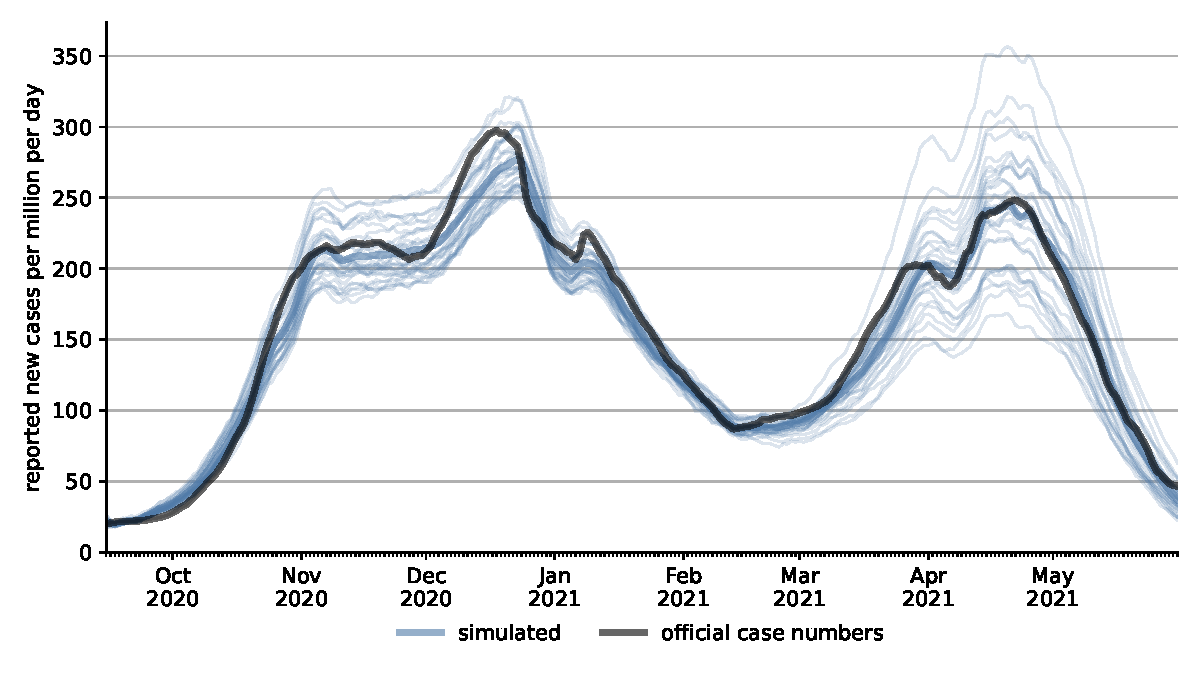
\includegraphics[width=\textwidth]{figures/results/figures/scenario_comparisons/combined_fit/full_new_known_case_with_single_runs}
  \caption{Fit Over the Full Simulation Time Frame with Single Simulation Runs}
  \floatfoot{\noindent \textit{Note:} The figure shows the weekly incidence rates per
  100,000 people for the reported simulated infections rates. The mean infection rate is
  the thick blue line. Single simulation runs are plotted in lighter and thinner lines.
  The official case numbers as reported by the Robert-Koch-Institut are plotted in black.
  The fit is overall very good. The higher the mean incidence and the stronger the growth
  the more variance there is between simulation runs. We averaged over 30 simulation
  runs.}
  \label{fig:aggregated_fit2}
\end{figure}

\begin{figure}[ht]
  \centering
  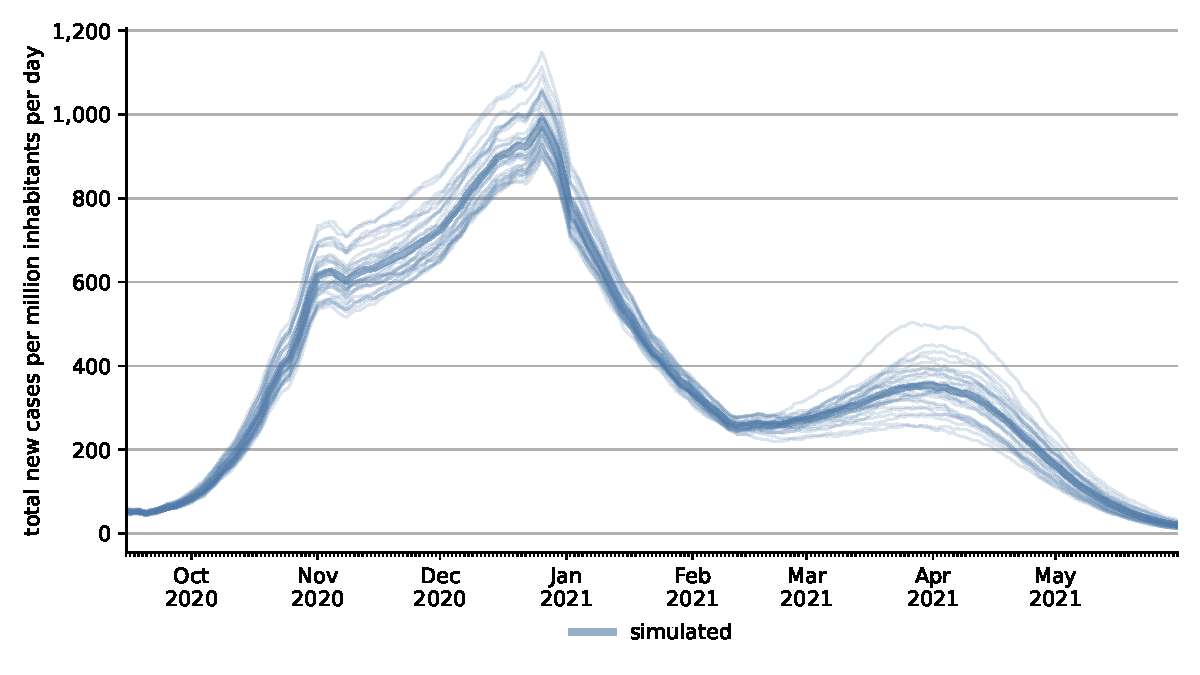
\includegraphics[width=\textwidth]{figures/results/figures/scenario_comparisons/combined_fit/full_newly_infected_with_single_runs}
  \caption{Development of the Total Infections Over the Full Simulation Time Frame with
  Single Simulation Runs}
  \floatfoot{\noindent \textit{Note:} The figure shows the true weekly incidence rates
  per 100,000 people, including undetected cases. The mean infection rate is the thick
  blue line. Single simulation runs are plotted in lighter and thinner lines. The higher
  the mean incidence and the stronger the growth the more variance there is between
  simulation runs. We averaged over 30 simulation runs.}
  \label{fig:newly_infected_in_baseline}
\end{figure}




\begin{figure}[ht]
  \centering
  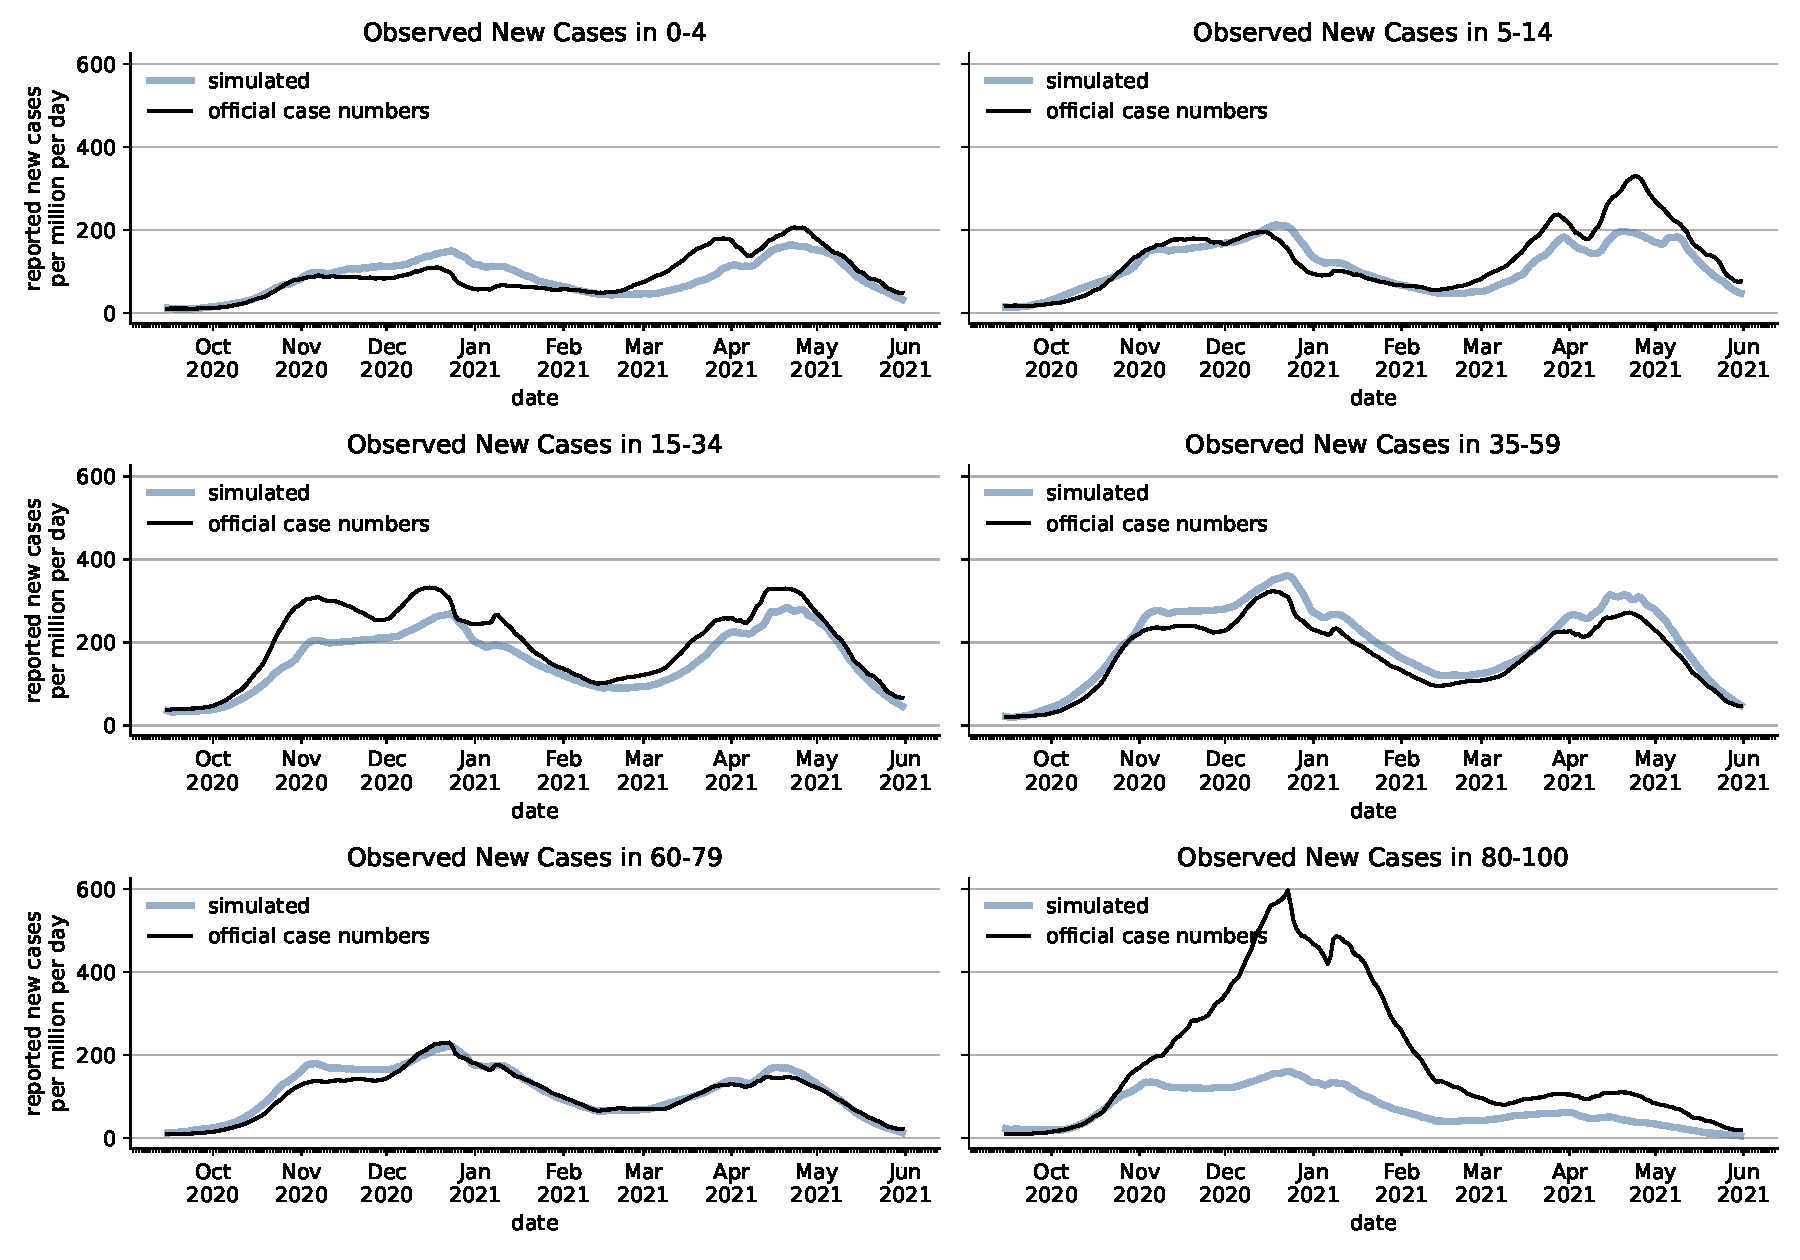
\includegraphics[width=\textwidth]{figures/results/figures/incidences_by_group/age_group_rki/full_combined_baseline_new_known_case}
  \caption{Simulated and Empirical Infections by Age Group}
  \floatfoot{\noindent \textit{Note:} The figure shows the weekly incidence rates per
  100,000 people for the reported versus the simulated infections rates for different age
  groups. The age group of individuals above 80 needs to be interpreted with caution
  because our synthetic population only includes private households, i.e. nursing homes
  are not represented in our model. They accounted for many cases and deaths in the
  winter of 2020 and many 80 to 100 year olds live in these facilities. However, the
  official data does not contain information on whether cases were nursing home
  inhabitants or not. We averaged over 30 simulation runs.}
  \label{fig:age_group_fit}
\end{figure}


\begin{figure}[ht]
  \centering
  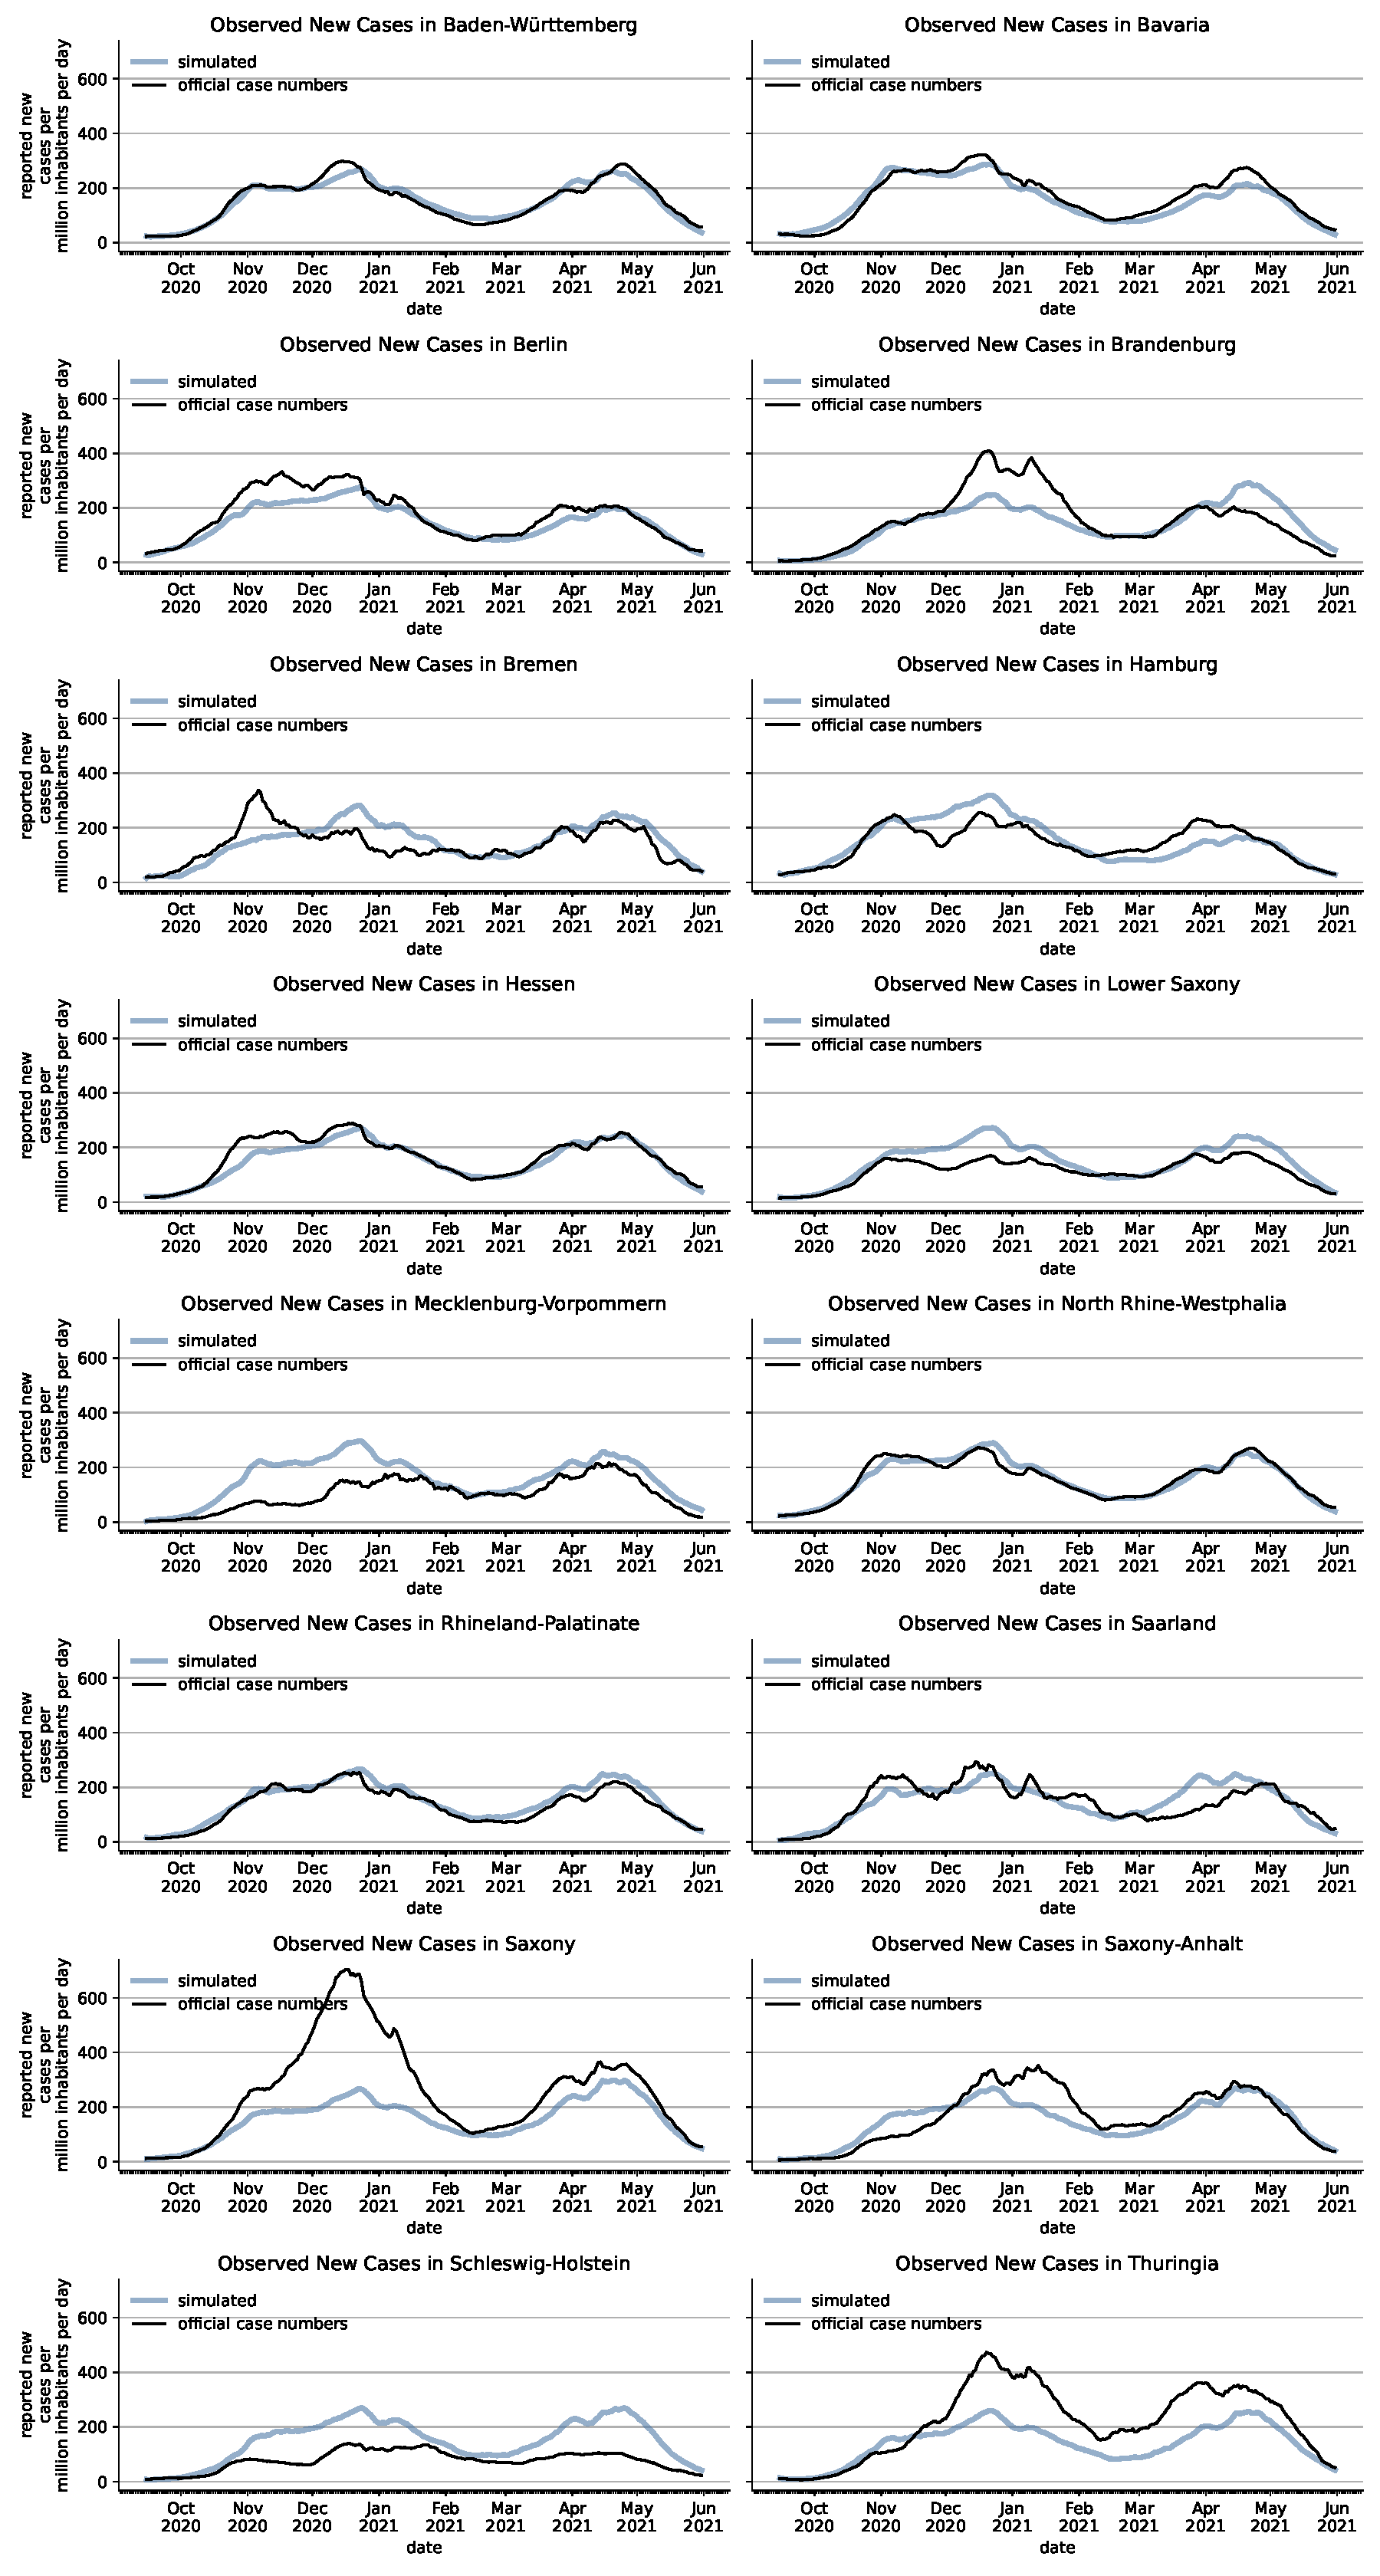
\includegraphics[width=\textwidth]{figures/results/figures/incidences_by_group/state/full_combined_baseline_new_known_case}
  \caption{Simulated and Empirical Infections by Federal State}
  \floatfoot{\noindent \textit{Note:} The figure shows the weekly incidence rates per
  100,000 people for the reported versus the simulated infections rates for different
  federal states. We averaged over 30 simulation runs.}
  \label{fig:state_fit}
\end{figure}


\begin{figure}[ht]
  \centering
  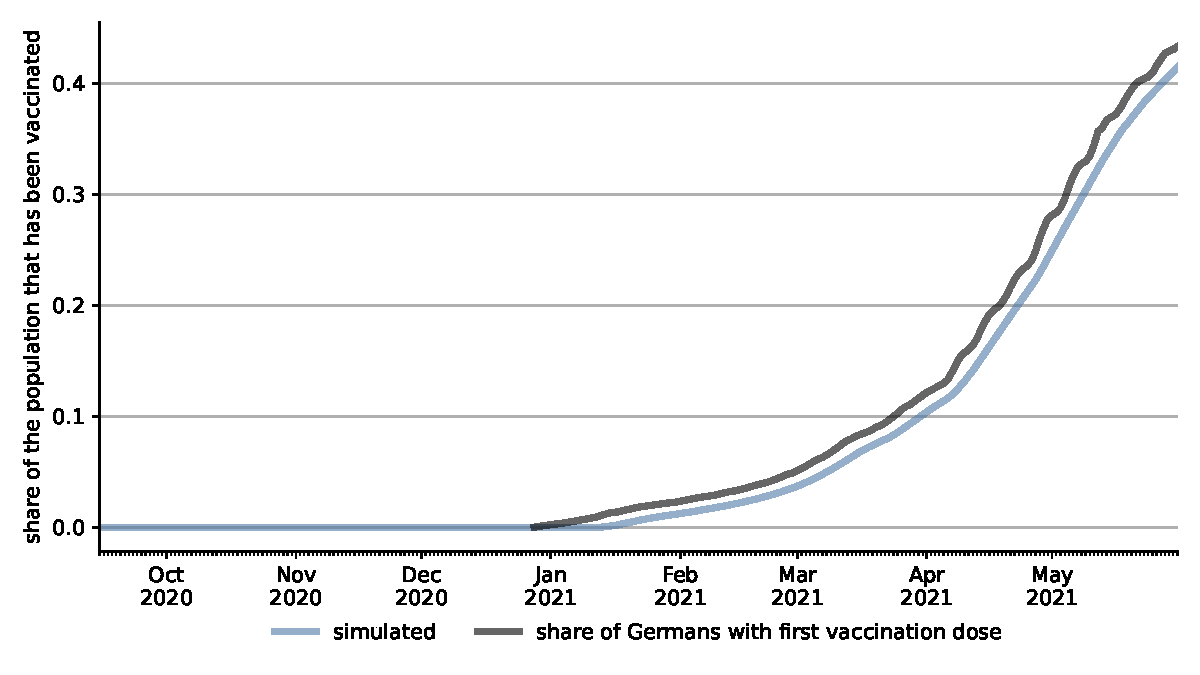
\includegraphics[width=\textwidth]{figures/results/figures/scenario_comparisons/combined_fit/full_ever_vaccinated}
  \caption{Share of Vaccinated Individuals}
  \floatfoot{\noindent \textit{Note:} The figure shows the rate of individuals that are
  vaccinated in our synthetic population versus in the general German population. Note
  that we excluded the vaccinations that were given to nursing homes, approximately the
  first percent of the German population that were vaccinated. Overall, our model covers
  a time frame that goes from zero vaccinated individuals to a state where over 40\% of
  the population are vaccinated. Our vaccinations work imperfectly but we do not model
  different vaccines nor do we distinguish between first and second shot.}
  \label{fig:fit_vaccinations}
\end{figure}


\begin{figure}[ht]
  \centering
  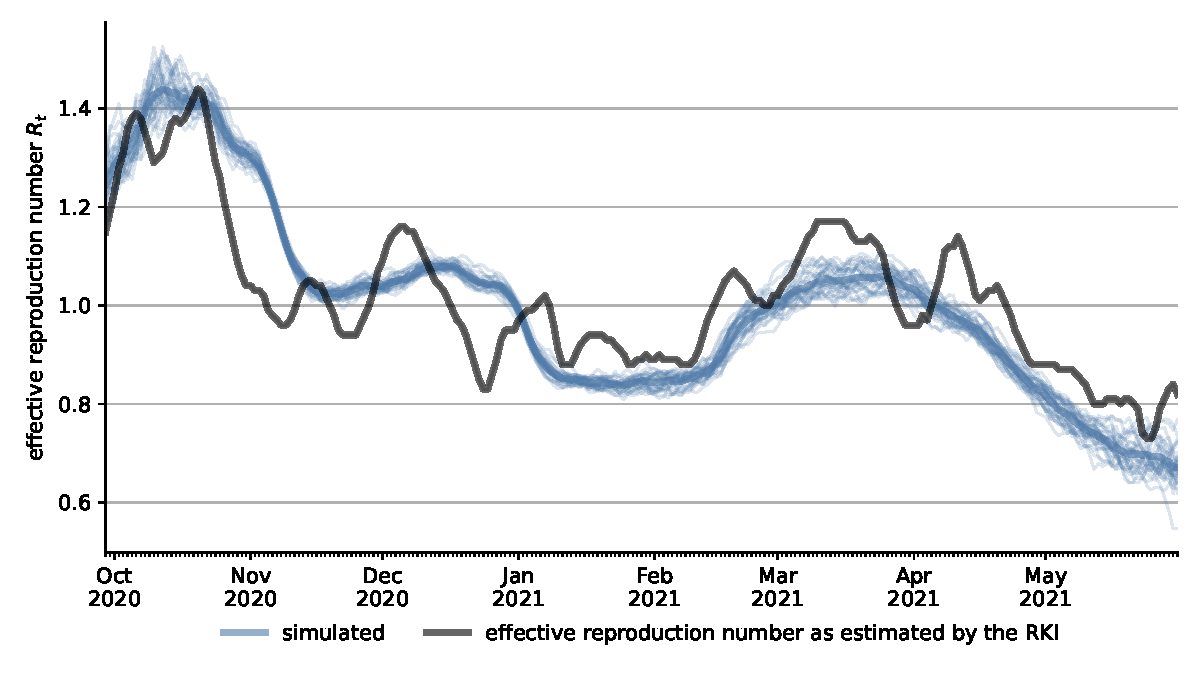
\includegraphics[width=\textwidth]{figures/results/figures/scenario_comparisons/combined_fit/full_r_effective_with_single_runs}
  \caption{Effective Replication Number $R_t$ in the Model and as Reported by the
  Robert-Koch-Institute}
  \floatfoot{\noindent \textit{Note:} The figure shows the effective replication number
  ($R_t$) as reported by the RKI and as calculated in our model. The $R_t$ gives the
  average number of new infections caused by one infected individual. The $R_t$ in our
  model broadly follows the $R_t$ reported by the RKI. Two trends stand out. Firstly, the
  RKI's $R_t$ drops faster in November. This could be due to a change in the testing
  policy that focused tests on the elderly when the second wave hit Germany and led to a
  decline in the overall share of detected cases. The second difference is from mid
  February to mid March where the RKI's reported $R_t$ increased more rapidly than that
  in our model. Here the opposite effect can be expected. During this time rapid tests
  increased strongly leading to more cases being detected. In the short term this leads
  an $R_t$ estimation that is based on detected cases to overestimate the replication
  number.}
  \label{fig:fit_r_effective}
\end{figure}


\begin{figure}[ht]
  \centering
  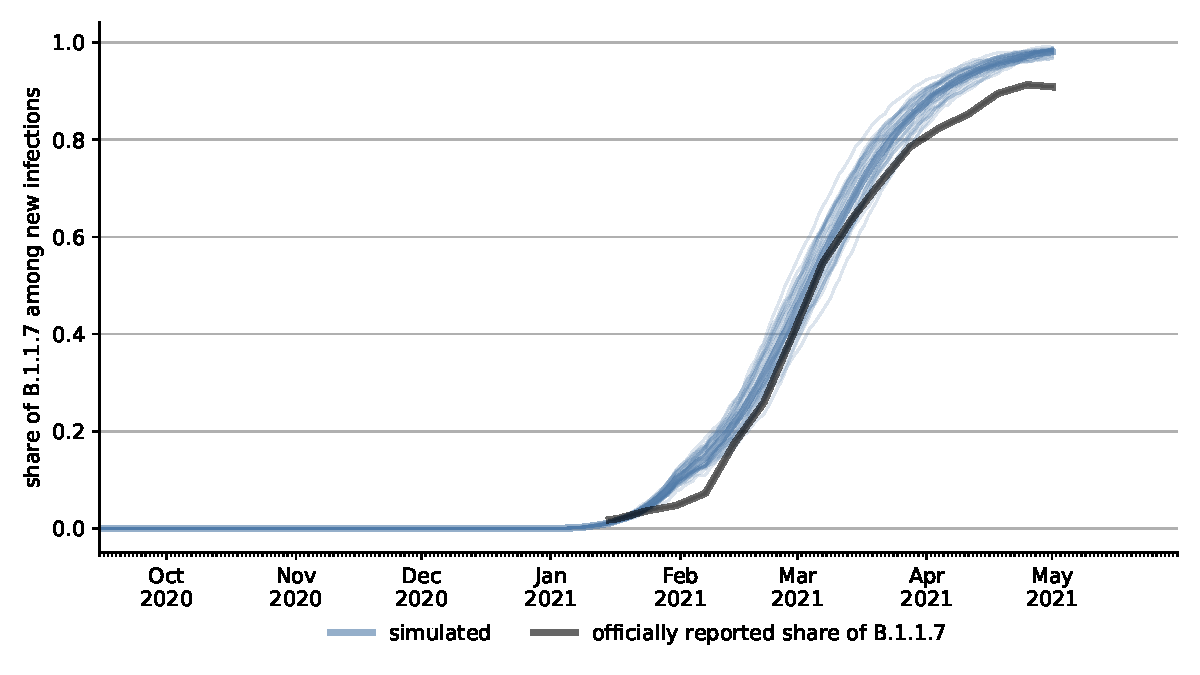
\includegraphics[width=\textwidth]{figures/results/figures/scenario_comparisons/combined_fit/full_share_b117_with_single_runs}
  \caption{Share of B.1.1.7 in the Model and as Reported by the Robert-Koch-Institute}
  \floatfoot{\noindent \textit{Note:} The figure shows the share of B.1.1.7 as
  reported by the RKI and as calculated in our model. We only introduce a few cases over
  the cause of January. From then B.1.1.7 takes over endogenously through its increased
  infectiousness. We model no other features of B.1.1.7. At most we introduce 0.75 cases per 100,000 inhabitants.}
  \label{fig:fit_share_b117}
\end{figure}




\FloatBarrier


\subsection{Share of Cases that are Detected}
\label{subsec:appendix_share_known_cases}

\begin{figure}[ht]
  \centering
  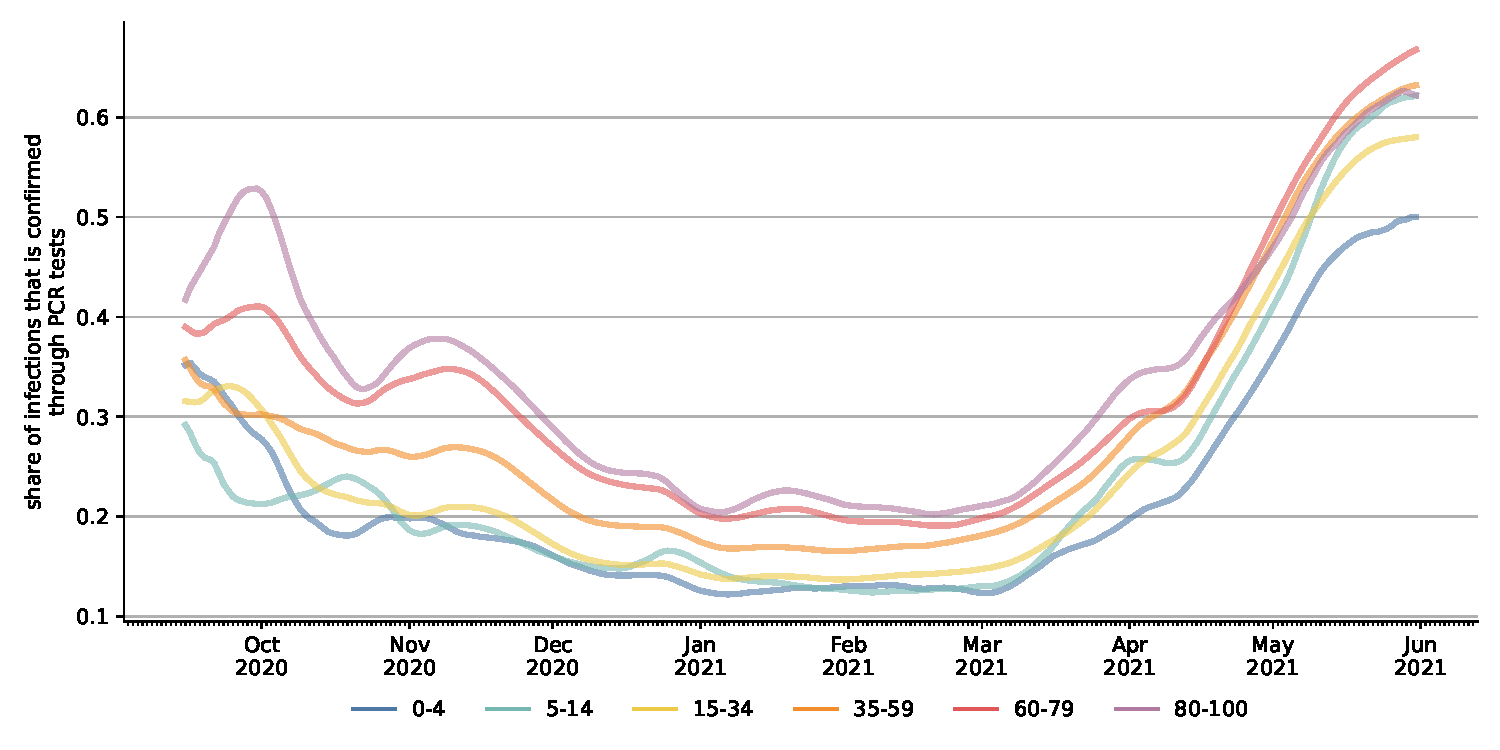
\includegraphics[width=\textwidth]{figures/results/figures/share_known_cases/full_combined_baseline_by_age_group_rki}
  \caption{Share of Detected Cases by Age Group}
  \label{fig:share_known_cases_by_age_group}
  \floatfoot{\noindent \textit{Note:} The figure shows the share of cases that is
  reported as an official case via PCR confirmation. We use the overall share of known
  cases that was estimated through the case fatality ratio by the
  \href{https://covid19.dunkelzifferradar.de/}{Dunkelzifferradar} for all of 2020 and
  then assume it to be constant as vaccinations of the elderly strongly affect the case
  fatality rate which the project does not account for. To get from an overall share of
  detected cases to the share of cases that is detected in each age group we use that
  asymptomatic cases are much less likely to be detected. As our model covers age
  specific asymptomatic rates this endogenously leads to group specific share known cases
  that verify that infections in younger age groups are under-detected. Starting in 2021
  in addition to the overall numbers of detected cases through symptoms and the share
  known cases, cases are also detected through confirmation of positive rapid tests. This
  leads to an increase in the share of known cases for all age groups but in particular
  for the younger age groups that are covered extensively with rapid tests through the
  rapid test requirement for participating in school.}
\end{figure}

It's noteworthy that the share of detected cases increases rapidly in May for the five to
fourteen year olds. This is a direct result of the mandatory tests in
school.

\subsection{Rapid Tests}
\label{subsec:appendix_rapid_tests}

\begin{figure}[ht]
  \centering
  \begin{subfigure}[b]{0.425\textwidth}
    \centering
    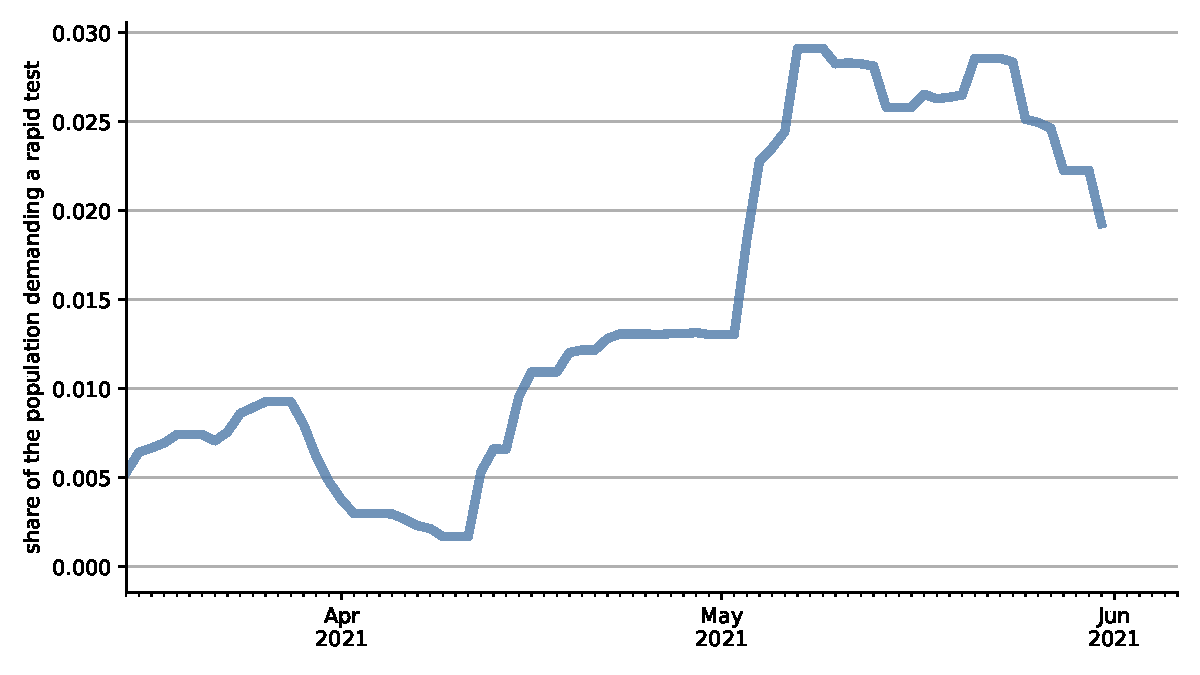
\includegraphics[width=\textwidth]{figures/results/figures/rapid_test_statistics/educ_demand_share}
    \caption{Share of the Population Demanding a Rapid Test in an Education Setting}
    \label{fig:educ_rapid_test_demand}
  \end{subfigure}
  \hfill
  \begin{subfigure}[b]{0.425\textwidth}
    \centering
    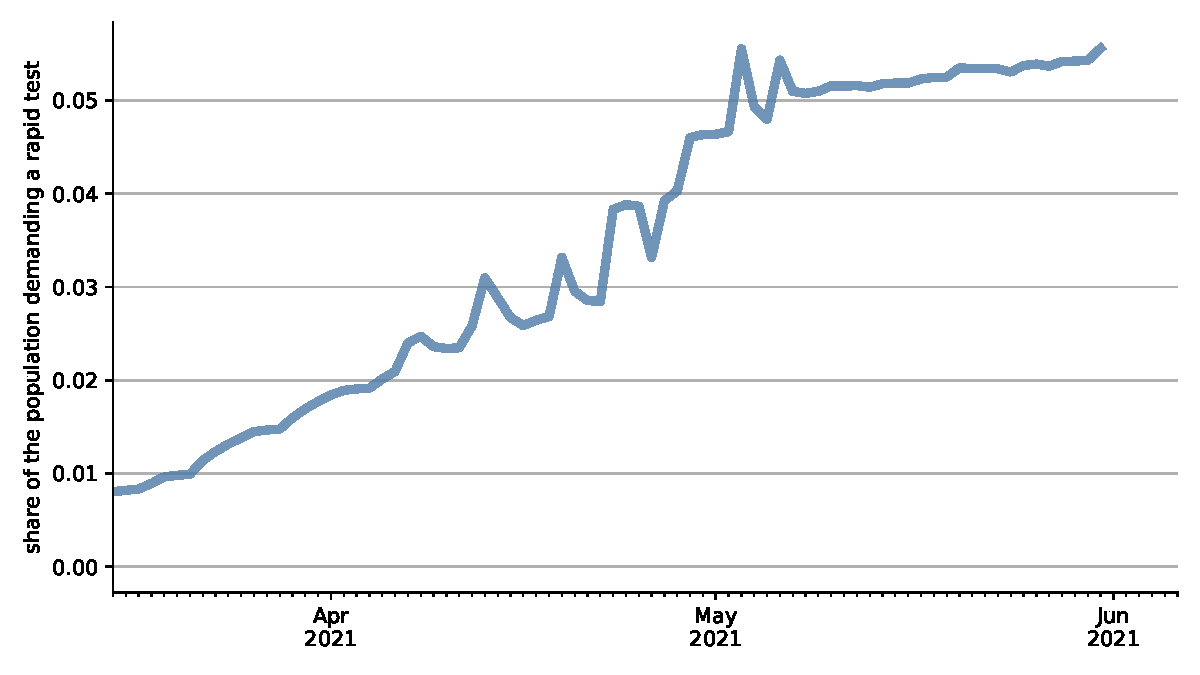
\includegraphics[width=\textwidth]{figures/results/figures/rapid_test_statistics/work_demand_share}
    \caption{Share of the Population Demanding a Rapid Test due to Work}
    \label{fig:work_rapid_test_demand}
  \end{subfigure}
  \hfill
  \begin{subfigure}[b]{0.425\textwidth}
    \centering
    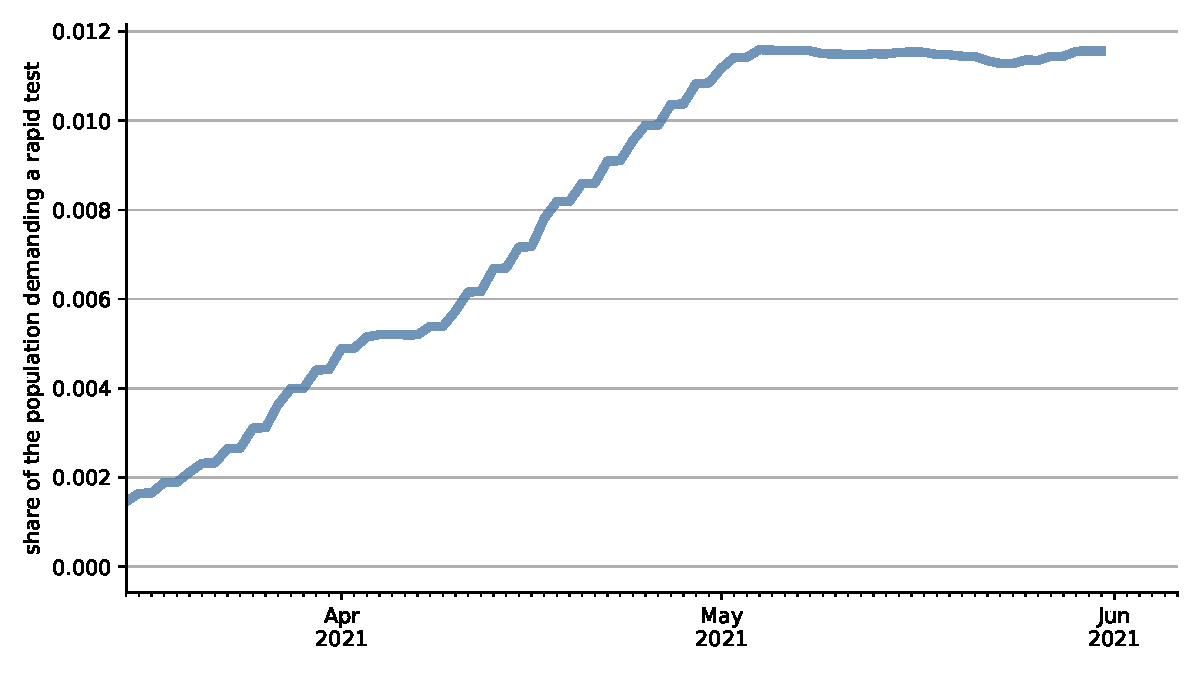
\includegraphics[width=\textwidth]{figures/results/figures/rapid_test_statistics/private_demand_share}
    \caption{Share of the Population Demanding a Rapid Test for Private Reasons}
  \label{fig:private_rapid_test_demand}
  \end{subfigure}
  \caption{Rapid Test Demand by Reason}
  \label{fig:rapid_test_demand_by_reason}
  \floatfoot{\noindent \textit{Note:}
    Rapid tests in the education setting are demanded by teachers (nursery, preschool and
    school) as well as school pupils. After Easter the required frequency of tests is
    increased from once per week to twice per week. Work rapid tests are demanded by
    individuals that still have work contacts, i.e. do not work from home. The share of
    employers offering rapid tests increases over the time frame and the frequency of
    testing is also increased. Tests are demanded by individuals for one of three private
    reasons: having developed symptoms without access to a PCR test, having a household
    member that has tested positive or developed symptoms or having planned weekly
    meeting with friends.
  }
\end{figure}


\begin{figure}[ht]
  \centering
  \begin{subfigure}[b]{0.425\textwidth}
    \centering
    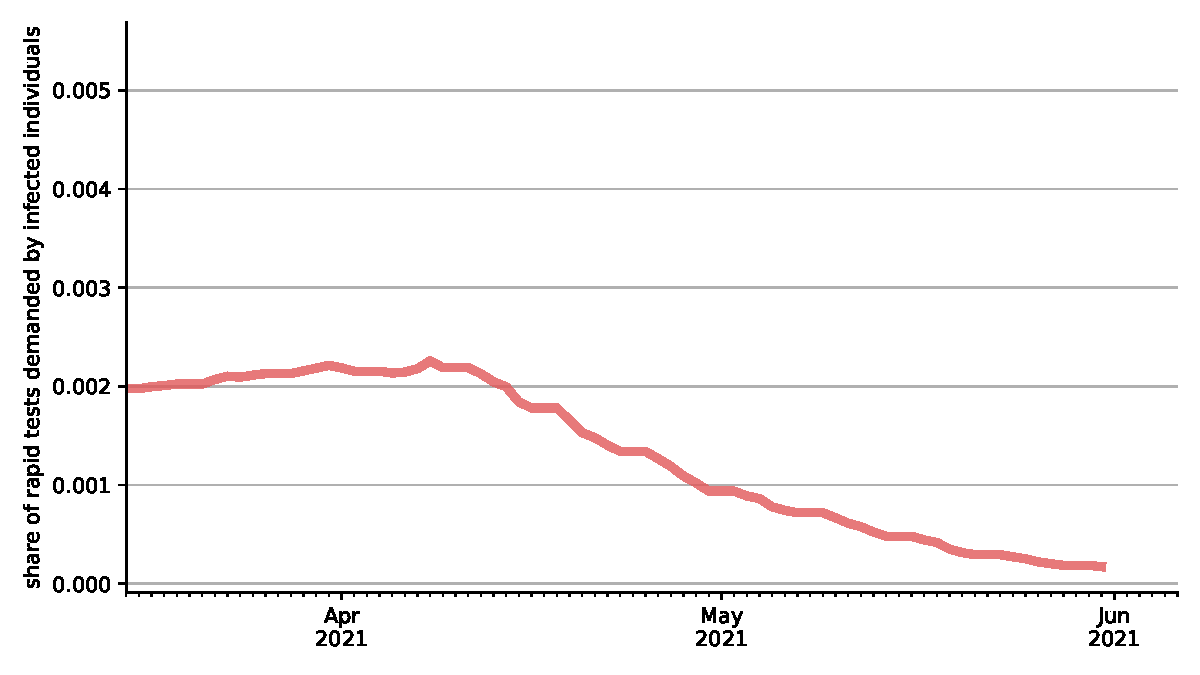
\includegraphics[width=\textwidth]{figures/results/figures/rapid_test_statistics/share_infected_among_educ_demand}
    \caption{Share of Rapid Tests in the Educational Setting Demanded by Infected
    Individuals}
    \label{fig:share_infected_among_educ_rapid_test_demand}
  \end{subfigure}
  \hfill
  \begin{subfigure}[b]{0.425\textwidth}
    \centering
    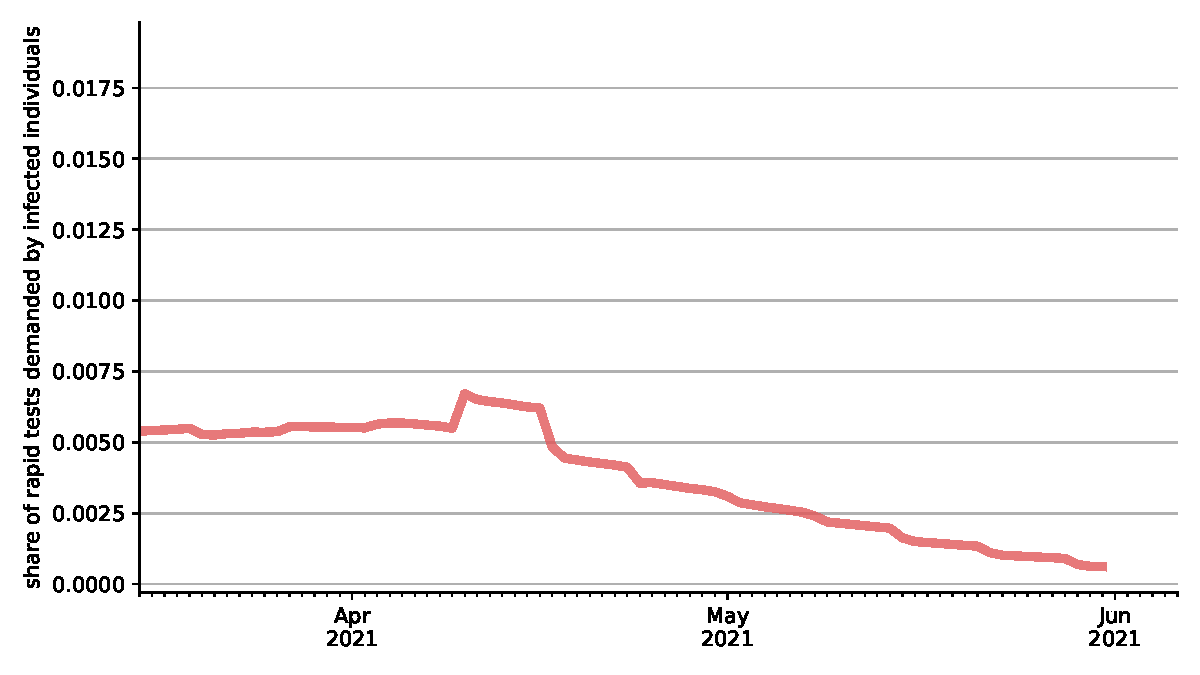
\includegraphics[width=\textwidth]{figures/results/figures/rapid_test_statistics/share_infected_among_work_demand}
    \caption{Share of Work Rapid Tests Demanded by Infected Individuals}
    \label{fig:share_infected_among_work_rapid_test_demand}
  \end{subfigure}
  \hfill
  \begin{subfigure}[b]{0.425\textwidth}
    \centering
    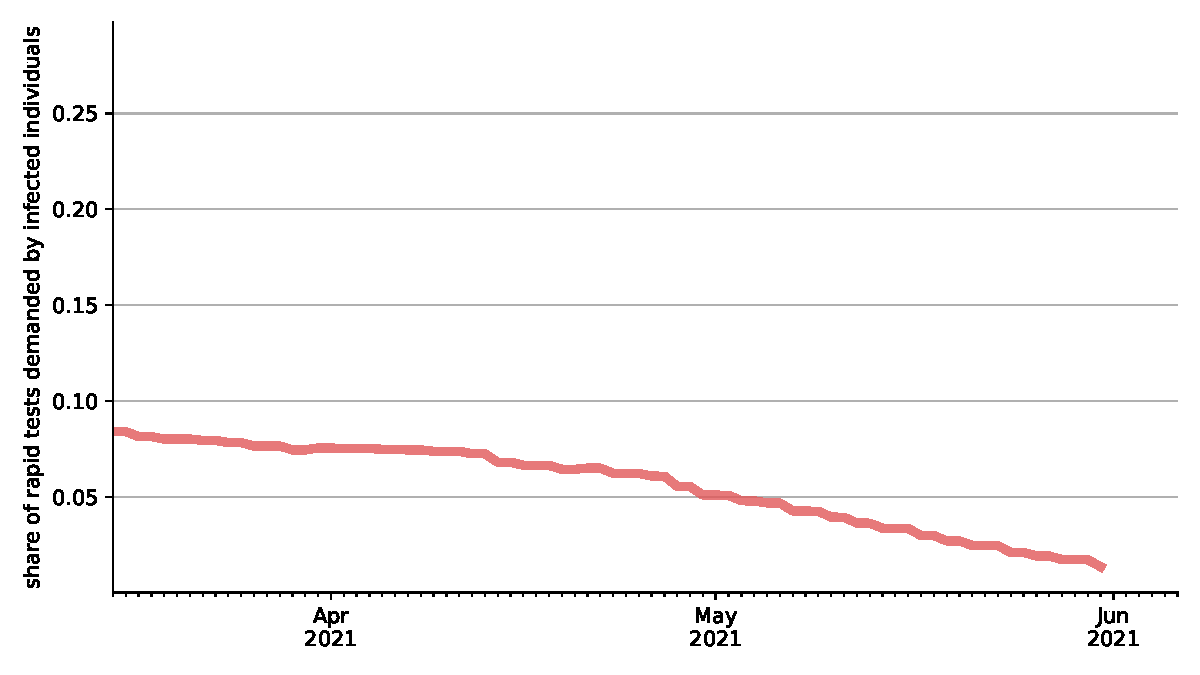
\includegraphics[width=\textwidth]{figures/results/figures/rapid_test_statistics/share_infected_among_private_demand}
    \caption{Share of Private Rapid Tests Demanded by Infected Individuals}
  \label{fig:share_infected_among_private_rapid_test_demand}
  \end{subfigure}
  \caption{Share of Rapid Tests Demanded by Infected Individuals by Reason}
  \label{fig:share_infected_among_rapid_test_demand_by_reason}
  \floatfoot{\noindent \textit{Note:}
    Rapid tests in the education setting are demanded by teachers (nursery, preschool and
    school) as well as school pupils. After Easter the required frequency of tests is
    increased from once per week to twice per week. Work rapid tests are demanded by
    individuals that still have work contacts, i.e. do not work from home. The share of
    employers offering rapid tests increases over the time frame and the frequency of
    testing is also increased. Tests are demanded by individuals for one of three private
    reasons: having developed symptoms without access to a PCR test, having a household
    member that has tested positive or developed symptoms or having planned weekly
    meeting with friends. Private rapid tests have a much higher share of infected
    individuals because they are mostly triggered by events that make an infection
    likely. Remember however, that one reason is that a household member has a positive
    rapid test. This means that work and education rapid tests which have a low rate of
    infected individuals trigger more targeted rapid tests through the household demand.
    They also have a much higher volume of tests. As can be seen in the decomposition
    (Figure~\ref{fig:2021_scenarios_decomposition_tests} every category of tests is
    important for the overall effect. It appears that the combination of wide testing to
    find infection chains plus targeted tests to break those chains taking together
    is important.}
\end{figure}






\FloatBarrier


\subsection{Scenarios}
\label{subsec:appendix_scenarios}


\begin{figure}[ht]
  \centering
  \begin{subfigure}{.6\textwidth}
    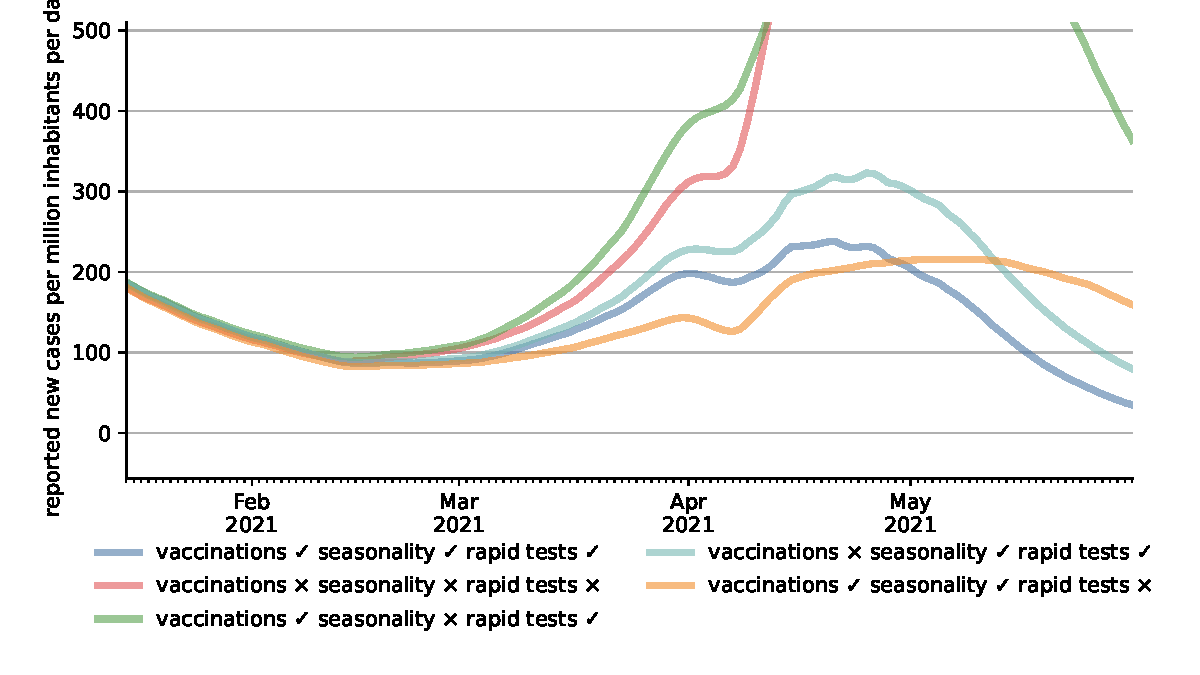
\includegraphics[width=0.9 \textwidth]{figures/results/figures/scenario_comparisons/one_off_and_combined/full_new_known_case_cropped}
  \end{subfigure}%
  \begin{subfigure}{.6\textwidth}
    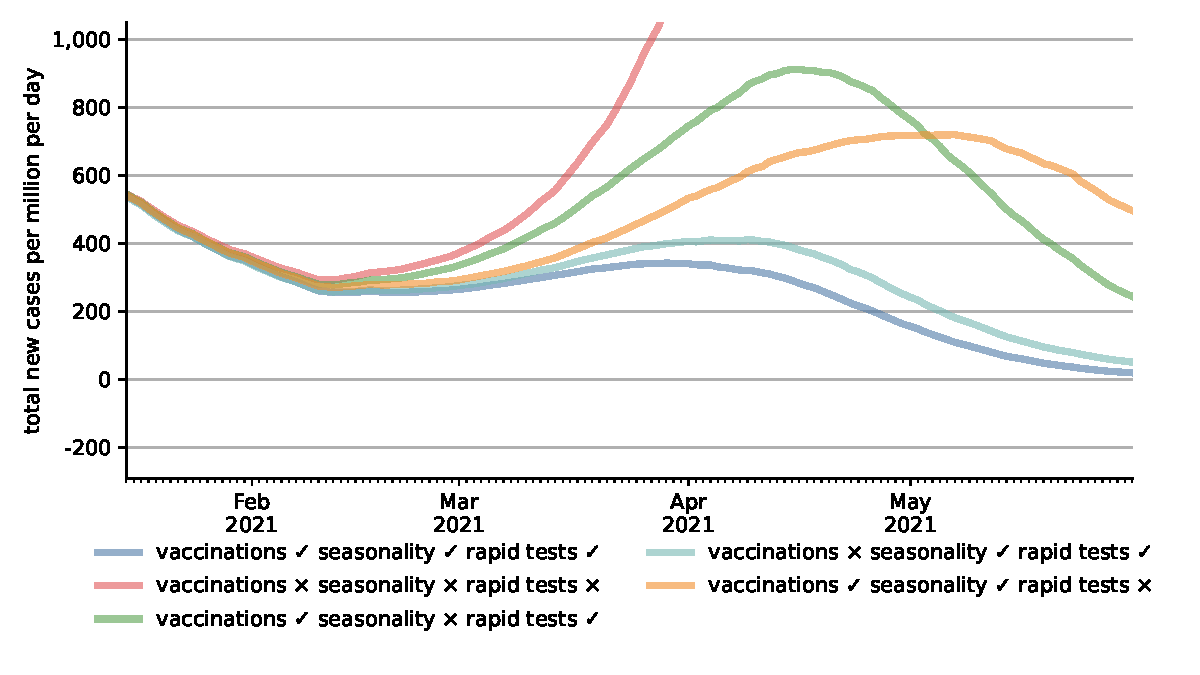
\includegraphics[width=0.9 \textwidth]{figures/results/figures/scenario_comparisons/one_off_and_combined/full_newly_infected_cropped}
  \end{subfigure}
  \caption{The Effect of Policies on Observed and Unobserved Cases}
  \label{fig:explain_decline}
  \floatfoot{\noindent \textit{Note:} \ldots}
\end{figure}



\begin{figure}[ht]
  \centering
  \begin{subfigure}{.6\textwidth}
    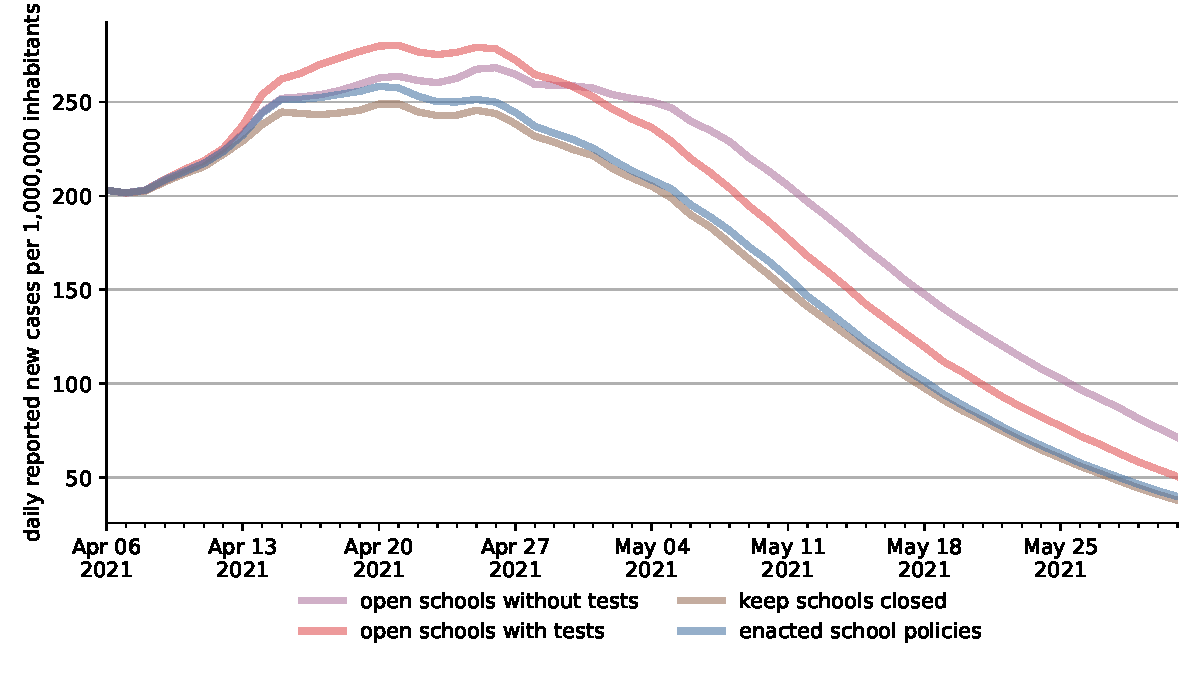
\includegraphics[width=0.9 \textwidth]{figures/results/figures/scenario_comparisons/school_scenarios/full_new_known_case}
  \end{subfigure}%
  \begin{subfigure}{.6\textwidth}
    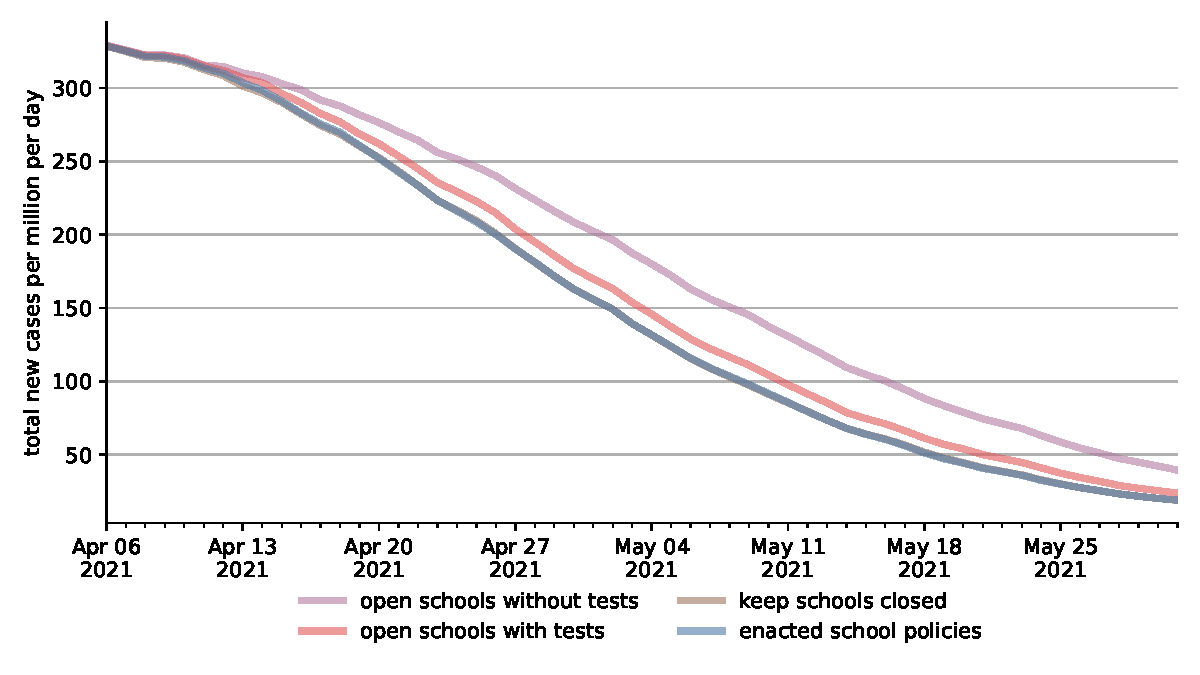
\includegraphics[width=0.9 \textwidth]{figures/results/figures/scenario_comparisons/school_scenarios/full_newly_infected}
  \end{subfigure}
  \caption{The Effect of Different School Scenarios on Observed and Unobserved Cases}
  \label{fig:school_scenarios_detailed}
\end{figure}


\FloatBarrier
